
\chapter{Design and Implementation}
\label{cha:implementation}

\section{Decomposition Algorithm}

Decomposition describes the task of grouping data fields into services. Achieving a good solution according to the defined Coupling Criteria as described in \ref{sec:decompositionRequirements} requires a non trivial algorithm. This section documents the evaluation process for such an algorithm.

\subsection{Approach \#1: Clustering of a Weighted Undirected Graph}
\label{subsec:approach1_graph}

Our first approach to solve the decomposition problem was using a weighted, undirected graph with a clustering or community algorithm. 

Every data field in the model is represented by a node. Edges define a relationship between two data fields. The weight on each edge shows how \textit{close} or \textit{cohesive} two fields are. The higher the weight, the more likely they should belong to the same service. Figure \ref{fig:weighted_graph} shows an abstract example of such a graph.

\begin{minipage}[t]{0.5\textwidth}
	Figure \ref{fig:graph_approach} outlines a solution sketch for this approach. As user representations are imported, data fields and  information for predefined Coupling Criteria are extracted by the \textit{Importer} to store all important information to create the graph.
	
	The \textit{Solver} then creates all vertices from the data fields and builds edges between them according to the stored Coupling Criteria instances. This task contains complexity for the following reasons:
	
	\begin{enumerate}
		\item Coupling Criteria are not homogeneous as described in Section \ref{subsec:couplingCriteriaTypes}. 
		%TODO: write first about types before completing this item. Mention distance, closeness and cumulative criteria
		
		\item All Coupling Criteria information is reduced to a single number with one single unit of measurement. An increase of the weight for one Criteria automatically changes the relative importance of that CC to others.
		
		\item To give the user a way to define the specific requirements of his system, priorities per Coupling Criteria can optionally be defined to influence the weights of each Coupling Criteria instance. 
	\end{enumerate}
	
	The \textit{Clustering Algorithm} then analyzes the graph and creates clusters of data fields so that as few edges as possible need to be cut.
	
	\begin{figure}[H]
		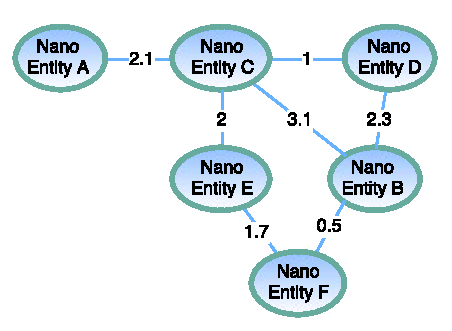
\includegraphics[scale=1.0]{diagrams/weighted_graph.pdf}
		\caption{Example of a Weighted Graph}
		\label{fig:weighted_graph}
	\end{figure}

\end{minipage}
\begin{minipage}[t]{0.5\textwidth}
	\begin{figure}[H]
		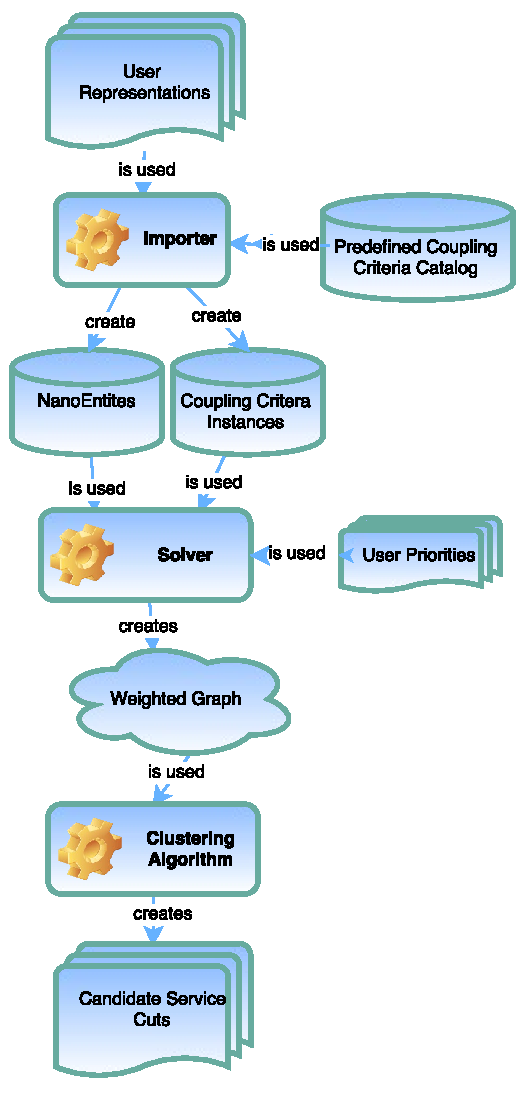
\includegraphics[scale=1.0]{diagrams/graph_approach.pdf}
		\caption{Solution Sketch for a Weighted Graph with a Clustering Algorithm}
		\label{fig:graph_approach}
	\end{figure}
\end{minipage}

A detailed evaluation of clustering algorithms is document in Appendix \ref{appendix:graphClustering}. We decided to do a first assessment of this approach with the MCL\cite{mcl} and Girvan-Newman\cite{girvanNewman} algorithms. Both algorithms are implemented as plugins of the Gephi\cite{gephi} platform and can be extracted as \gls{JAR} files.

\subsubsection{Practical Assessment of the Graph Clustering Approach}

To assess the graph approach we use a simple booking domain model. In Figure \ref{fig:clusteringBookingSimple} the MCL algorithm was run on the booking model with all Coupling Criteria priorities set to zero expect the Variant \textit{Same Entity} of the \textit{Identity \& Lifecycle Commonality} Criteria. Consequently the visualized Services contain one entity each. The entities can be identified as \textit{Customer}, \textit{Article} and \textit{Customer}.

\begin{figure}[H]
	\begin{center}
		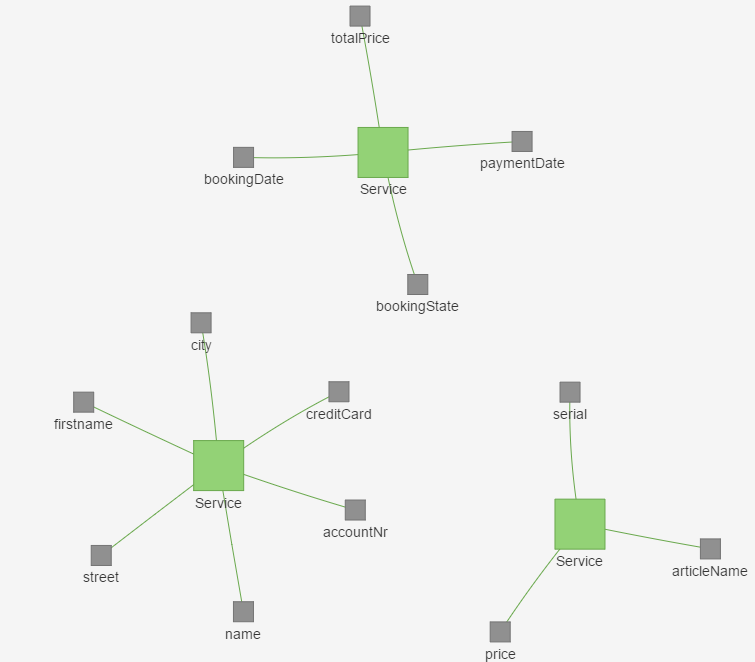
\includegraphics[scale=0.8]{images/booking_entities.png}
	\end{center}
	\caption{Clustering of a simple Booking example.}
	\label{fig:clusteringBookingSimple}
\end{figure}


Figure \ref{fig:clusteringBooking} shows the result of the MCL algorithm with user stories of the Booking domain added. 

\begin{figure}[H]
	\begin{center}
		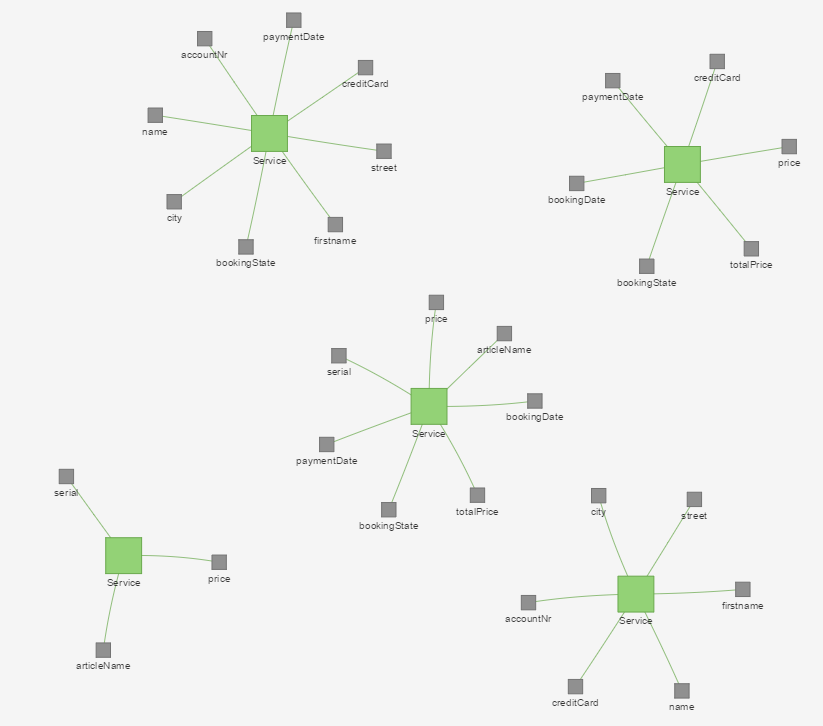
\includegraphics[scale=0.7]{images/booking_entities_mcl.png}
	\end{center}
	\caption{Booking Example enhanced with User Stories.}
	\label{fig:clusteringBooking}
\end{figure}

Obviously this is not the result expected. The requirement that a data field should be once and only once grouped to a Service is not met and the meaning of each Service can't be interpreted. 


\subsubsection{Theoretical Assessment of the Graph Clustering Approach}
Theoretical assessment


\subsection{Approach \#2: Set Rating}



\begin{figure}[H]
	\begin{center}
		\includegraphics[scale=0.45]{diagrams/scoring_process.png}
	\end{center}
	\caption{Set based scoring process.}
	\label{fig:setProcess}
\end{figure}

\subsection{Approach \#3: Constructing Services - a Heuristic Approach}

\section{Prototype} 

\subsection{Design}

\subsection{Technology}

\subsection{Infrastructure}

\subsection{Information Security}

The web application is secured using an authentication and authorization implementation. Any other internal components such as the database or web services are hidden behind the servers firewall and therefore do not need any special security measures.

The uploaded data models are initially shared amongst all registered users.

\subsection{User Interface}

The base layout is responsive and adapts to smaller screens such as smartphones. However the tool is mostly used on devices such as laptops and the controls are therefore optimized for use on screens that are at least 15 inches wide and used with a mouse and a keyboard.


\bigskip
After covering the important design and implementation aspects, the next chapter assesses the built solution described in this chapter against the defined requirements.
